\section{Results}

%For results talk about what you would measure.

To determine the results of the experiment, I would conduct the experiment on each cockroach. Ideally, I would have at least 10 cockroaches to test on. For each experiment, I would use a timer to measure the time it took for a cockroach to react to the stimulation and the electrical tape to measure the angle of turn. 

% What else should I measure?

With the cockroaches that successfully turn left and right when stimulated, I will place them on track made of thin strips of electrical tape consisting of straight paths and \ang{90} turns and observe their ability to make it all the way through. I will also test the roach's ability to turn to various angles by modulating the current sent to its antennae and evaluating its performance of different maneuvers such as the Dieudonne Spiral, a zig-zag, and a sinusoid. % talk more about how it would execute the different maneuvers 

Once directional control is achieved, I will try to achieve speed control. Stimulation to the antennae may not necessarily control speed in addition to direction, so I will attempt to stimulate other areas of the roach's body to change its speed.

{\begin{figure}[ht!]
\centering
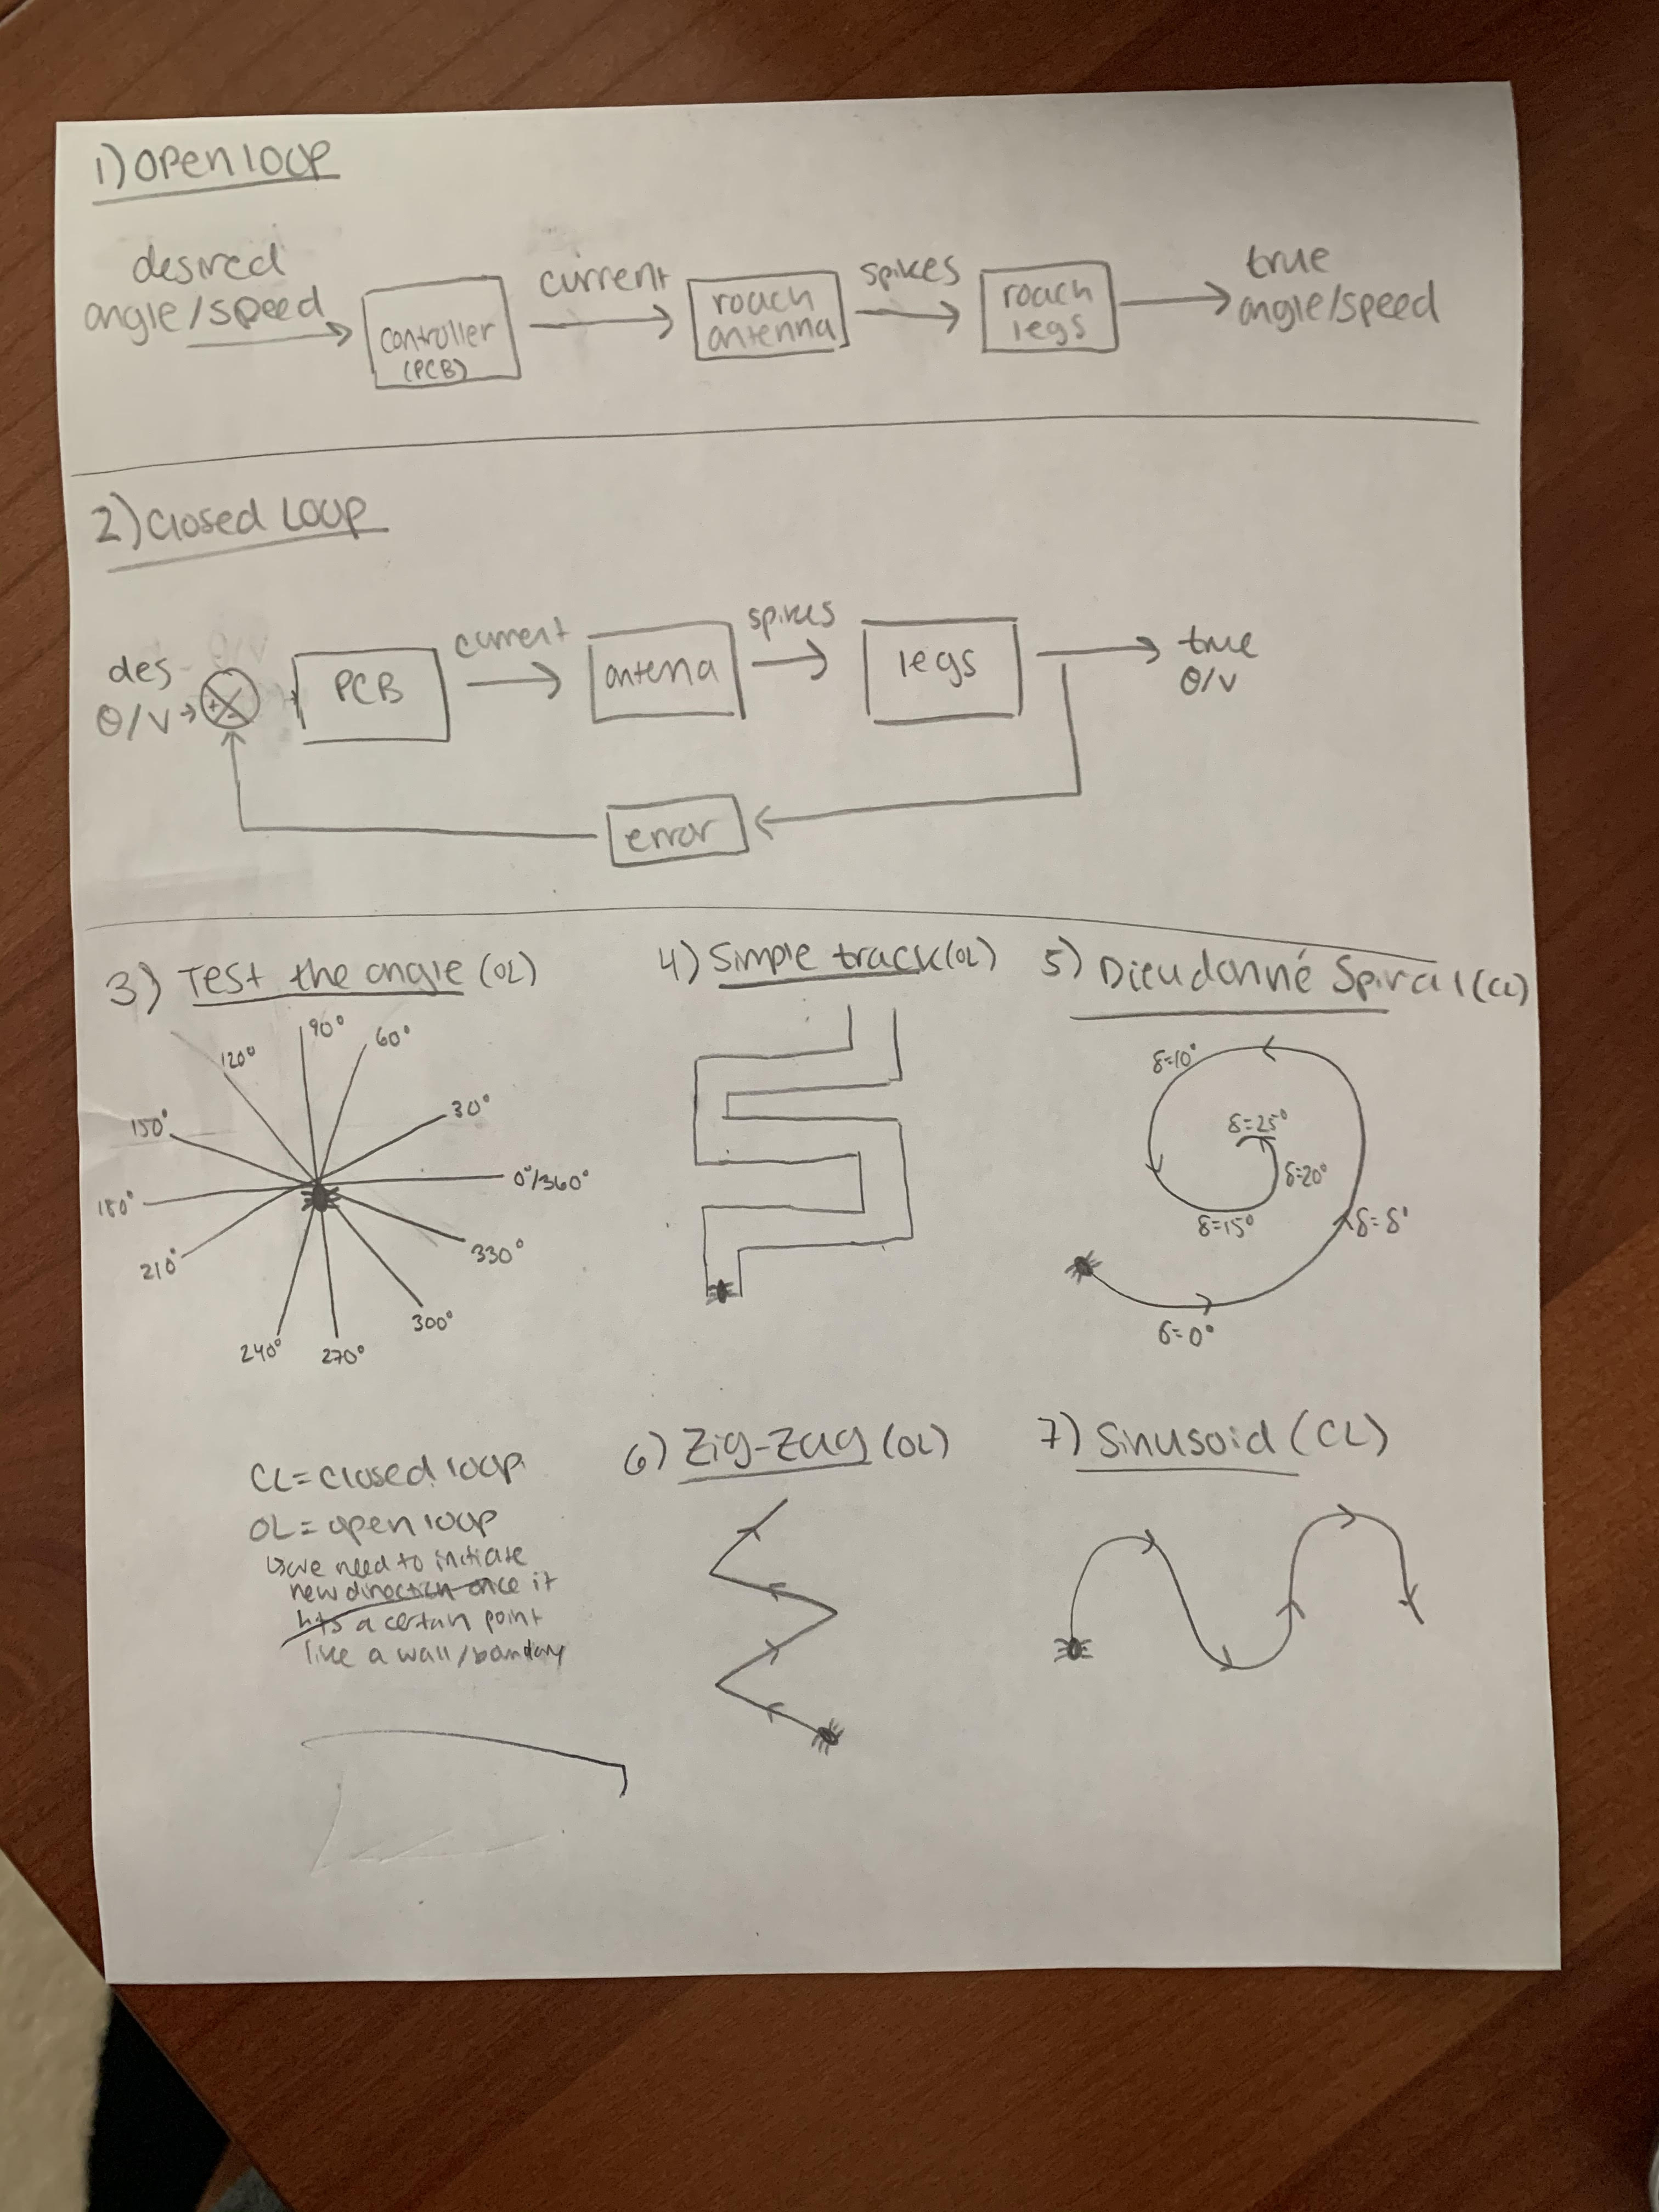
\includegraphics[scale=0.1]{Figures/OpenClosedLoops.jpg}
\caption{Rough ideas...feedback please?}
\label{fig:rough}
\end{figure}}


 